\begin{frame}{Reproducible Test Environment}
    \framesubtitle{A virtual enterprise network built with Containerlab}

    \begin{columns}[T,onlytextwidth]

        \begin{column}{0.62\textwidth}
                \centering
                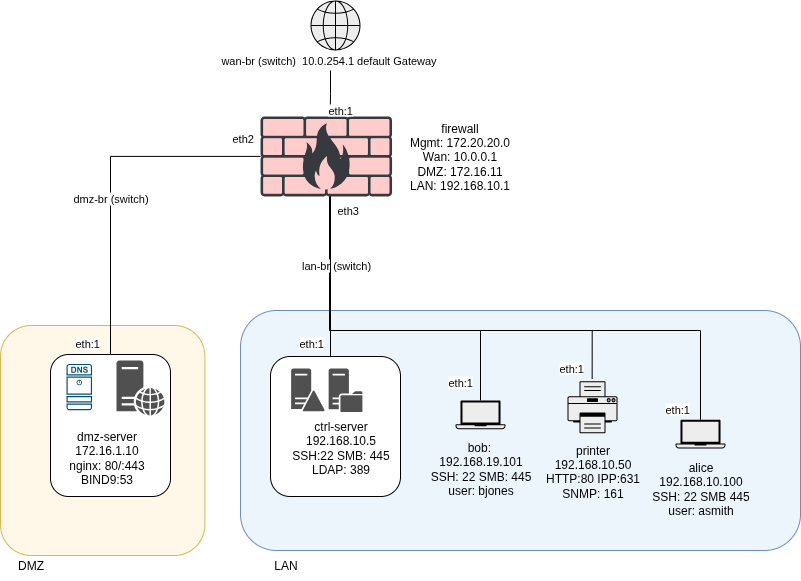
\includegraphics[width=\linewidth]{assets/test-topology}
        \end{column}

        \begin{column}{0.38\textwidth}


            \scriptsize
            \uncover<2->{
                \textbf{Why Containerlab?}
                \begin{itemize}
                    \item Reproducible topology from one config file
                    \item Multi-interface nodes \& fast teardown
                    \item Clean state per experiment
                \end{itemize}
            }
            \vspace{0.4em}
            \uncover<3-> {
                \textbf{Intentional vulnerabilities}
                \begin{itemize}
                    \item LDAP anonymous bind\\ + \textbf{cleartext creds} (\texttt{Password123!})
                    \item SMB signing not required; public share
                    \item SSH banners leak org name
                    \item DMZ: DNS zone transfer, \texttt{/secret.txt}
                \end{itemize}
            }

        \end{column}
    \end{columns}
\end{frame}


\begin{frame}{Evaluation Methodology}
    \framesubtitle{Models, environments and criteria}

    \begin{columns}[T,onlytextwidth]
        \begin{column}{0.5\textwidth}
            \textbf{Three models}
            \begin{itemize}
                \item[\faCloud] \texttt{claude-opus-4-7} \scriptsize frontier (Anthropic API)
                \item[\faServer] \texttt{gpt-oss:120b} \scriptsize open-weight, BFH-hosted
                \item[\faMicrochip] \texttt{qwen3:30b} \scriptsize local, self-hosted (Ollama)
            \end{itemize}

            \vspace{0.5em}
            \textbf{Three environments}
            \begin{itemize}
                \item \scriptsize Virtual (Containerlab) -- reproducible
                \item \scriptsize BFH Network Security Lab -- real network
            \end{itemize}
        \end{column}

        \begin{column}{0.5\textwidth}
            \begin{itemize}
                \item \textbf{Quantitative} \scriptsize duration, token usage, hosts / services / findings
                \item \textbf{Qualitative} \scriptsize correctness \& hallucination (1--10 scale), consistency
            \end{itemize}

            \vspace{0.5em}
            \begin{block}{\faChartBar~~Benchmark suite}
                \scriptsize
                \texttt{BenchmarkManager} runs each scenario $n$ times, resets state between runs,
                and aggregates a \texttt{BenchmarkReport} (JSON + Markdown) -- automating the quantitative metrics.
            \end{block}
        \end{column}
    \end{columns}
\end{frame}
